\chapter{Results}
\label{cha:results}

In this chapter are reported the results and the trends emerged from the created dashboards. It is shown how intuitive the comparison between different language is. For this purpose it is used a language sample taken from the major European languages, namely Italian, German, French and Spanish. They will be compared under the same vital sign to understand the explanatory power of these interactive visualizations and their potential role in the future steps of the Wiki Community Health Metrics project.
We remind that these measurements can be observed by everyone with the online dashboards\cite{vitalsign}, in order to study different languages from the one reported in this chapter. 

\section{Editors}
\label{sec:editors_conclusion}

We begin with Active editors. We remind they are the editors who edit Wikipedia pages at least five times per month. They are the majority of the editors, reaching up to 88\% of the total editors (considering the major language community). The dashboards show how the number of active editors evolved since the birth of Wikipedia until present days.

\begin{figure}[h]
    \centering
    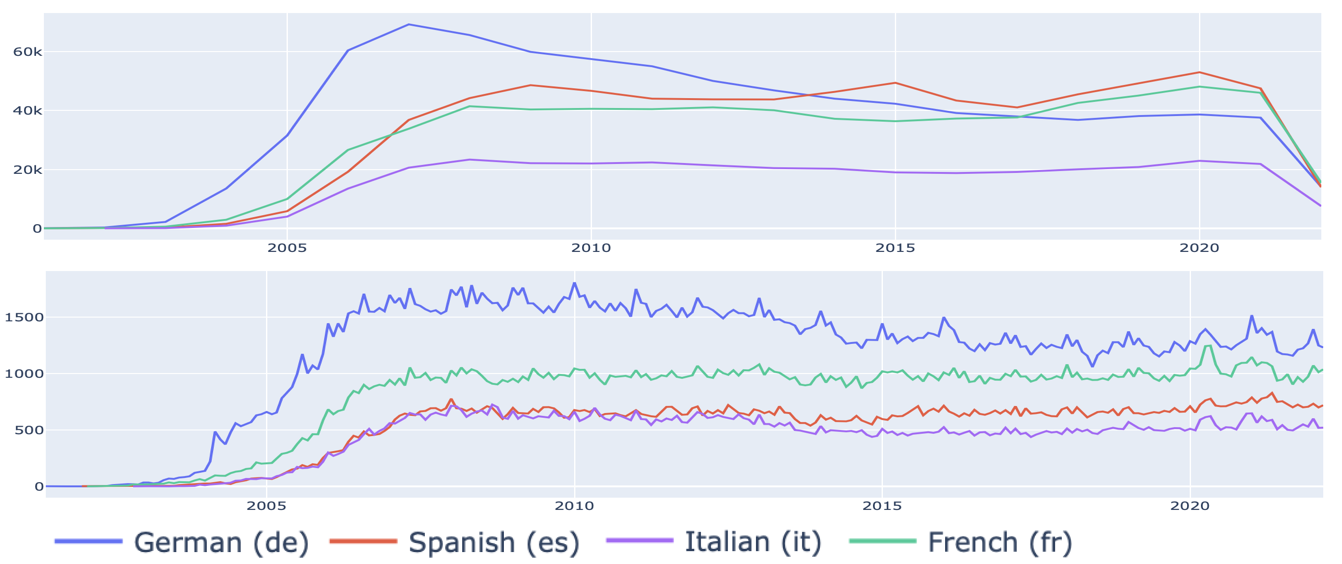
\includegraphics[width=470px]{img/editors_trend.png}
    \setlocalecaption{english}{figure}{Figure}
    \caption{Trend of the major European languages' active and very active editors}
    \label{fig:editors_trend}
\end{figure}

Considering a yearly visualization the first graph in Figure  \ref{fig:editors_trend} shows a general pattern for the major European language communities: after a rapid spike in the early days of Wikipedia, the number of active editors declined until, around the year 2014, they generally reached a stable value.\\
Considering the very active editors and monthly visualization, we get richer charts. The trend in Figure \ref{fig:editors_trend} stays the same but we can also see the number of very active editors fluctuating even during the years themselves: at the beginning of the new year the editors are more than the rest of the year.

\section{Retention}
\label{sec:retention_conclusion}

We now consider the retention dashboards considering the same language sample as before. We remind that the retention rate of a certain community is calculated as the percentage of new editors that survives after a certain threshold from their first edit. We consider the threshold value of 60 days.\\

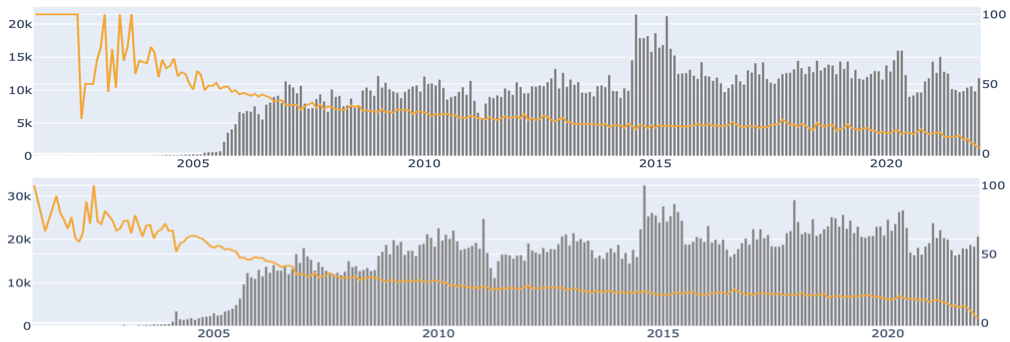
\includegraphics[width=470px]{img/retention_trend.png}
\pagebreak
\begin{figure}[h]
    \centering
    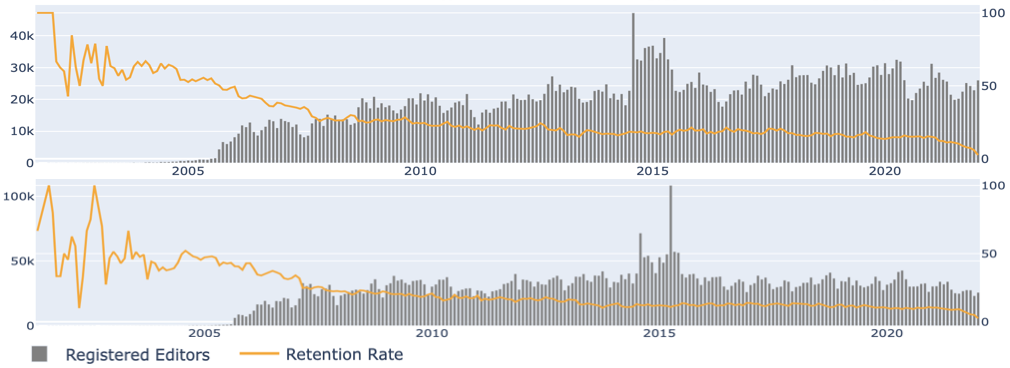
\includegraphics[width=470px]{img/retention_trend1.png}
    \setlocalecaption{english}{figure}{Figure}
    \caption{Trend of the major European languages' retention rates}
    \label{fig:retention_trend}
\end{figure}
\\
From top to bottom: Italian, German, French and Spanish.\\
The retention rates of our language sample show a dramatic declining trend. In every language we observe a common pattern: in the early days we can see a lot of instability, then around the year 2004 the retention rate steadily decreases, especially in the last years. Ideally, the various community should adopt behaviour to revert this trend.


\section{Stability}
\label{sec:stability_conclusion}

Before analyzing the stability trends we remind that the stability of the community is given by the persistence of active and very active editors, as well as by the succession of the various generations of editors over time.\\

\begin{figure}[h]
    \centering
    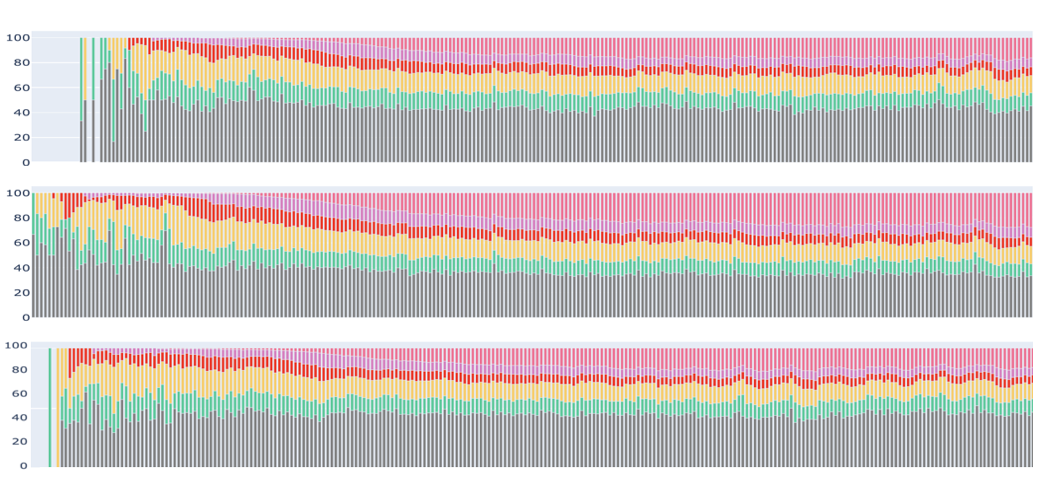
\includegraphics[width=460px]{img/stability_trend.png}
    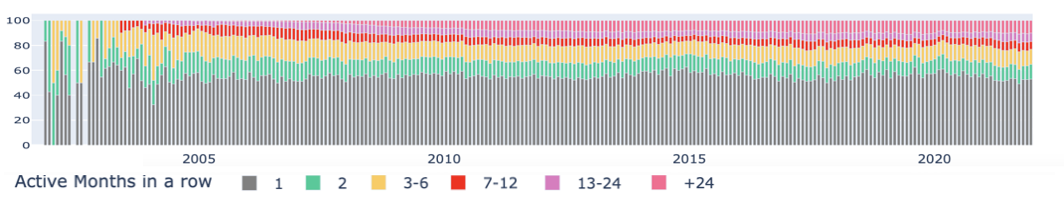
\includegraphics[width=460px]{img/stability_trend1.png}
    \setlocalecaption{english}{figure}{Figure}
    \caption{Trend of the major European languages' stability among active editors}
    \label{fig:stability_trend}
\end{figure}
\pagebreak

As seen in Figure \ref{fig:retention_trend} we have, from top to bottom, Italian, German, French and Spanish stability values.\\
Among active editors, the greater percentage of editors keeps editing for one month. Thus we could deduce that active editors tend to be volatile and less persistent. This trend is consistent across the whole language sample.\\

\begin{figure}[h]
    \centering
    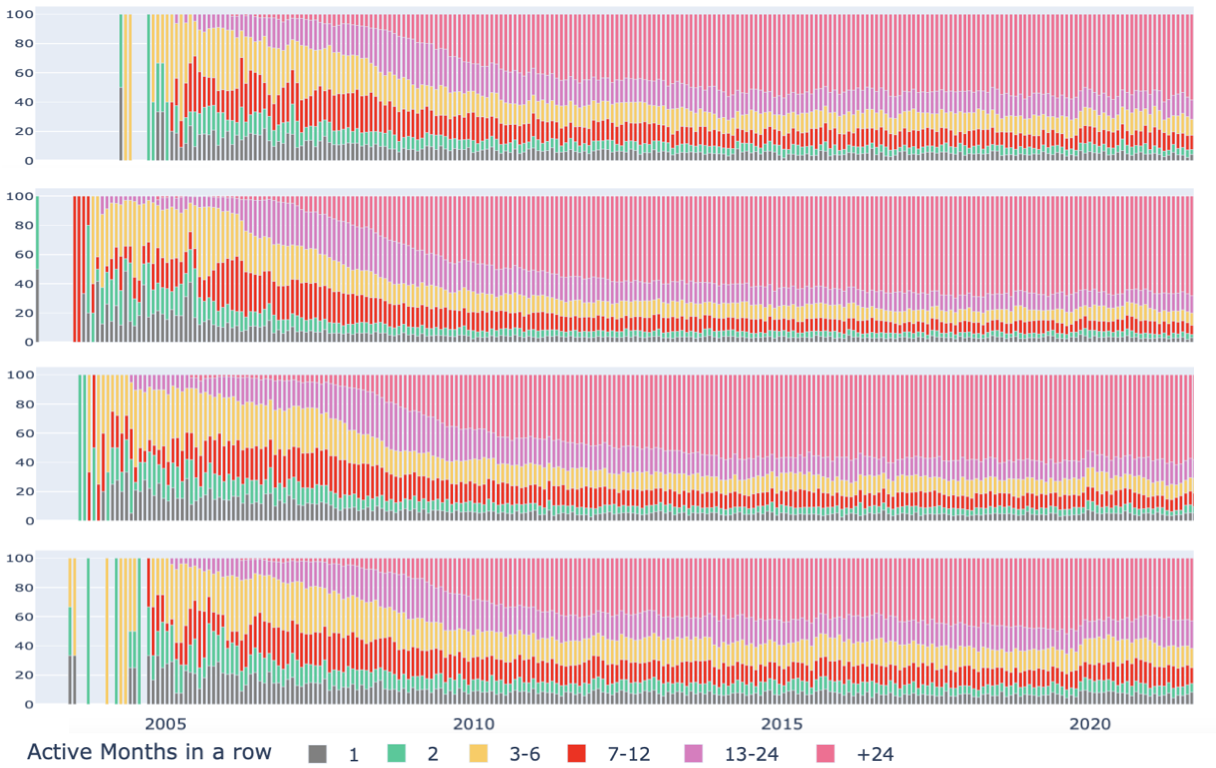
\includegraphics[width=480px]{img/stability_trend_v.png}
    \setlocalecaption{english}{figure}{Figure}
    \caption{Trend of the major European languages' stability among very active editors}
    \label{fig:stability_trend_v}
\end{figure}

While among the very active editors, the main part is represented by the editors which keep editing for more than 24 months. Since being a very active editor requires more effort than being simply active, we could argue that this very same effort pushes the editors towards being more and more dedicated to their role.\\
Ideally both fresh and long-term engaged editors should be present in every community.

\section{Balance}
\label{sec:balance_conclusion}

We now consider the balance visualizations. The Community balance metric measures the ability to maintain an equal proportion of old and new contributors.\\

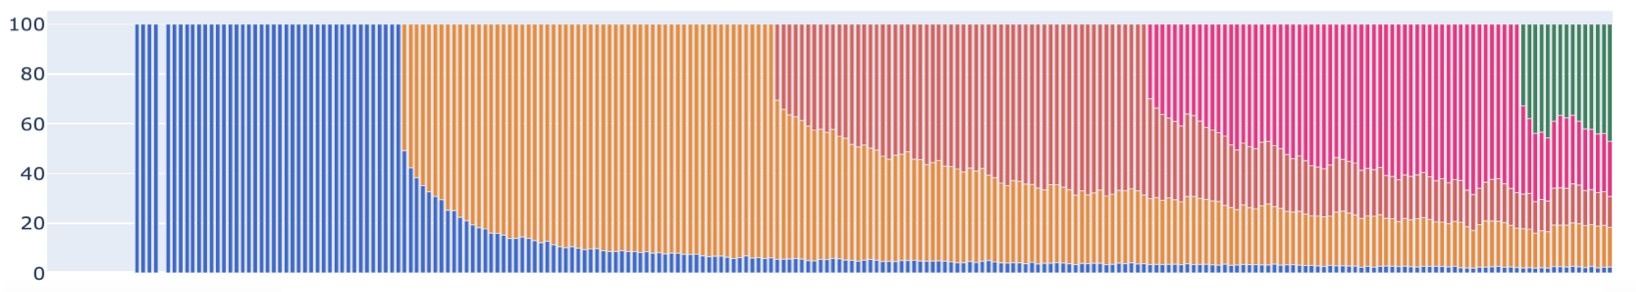
\includegraphics[width=470px]{img/balance_trend.png}
\pagebreak
\begin{figure}[h]
    \centering
    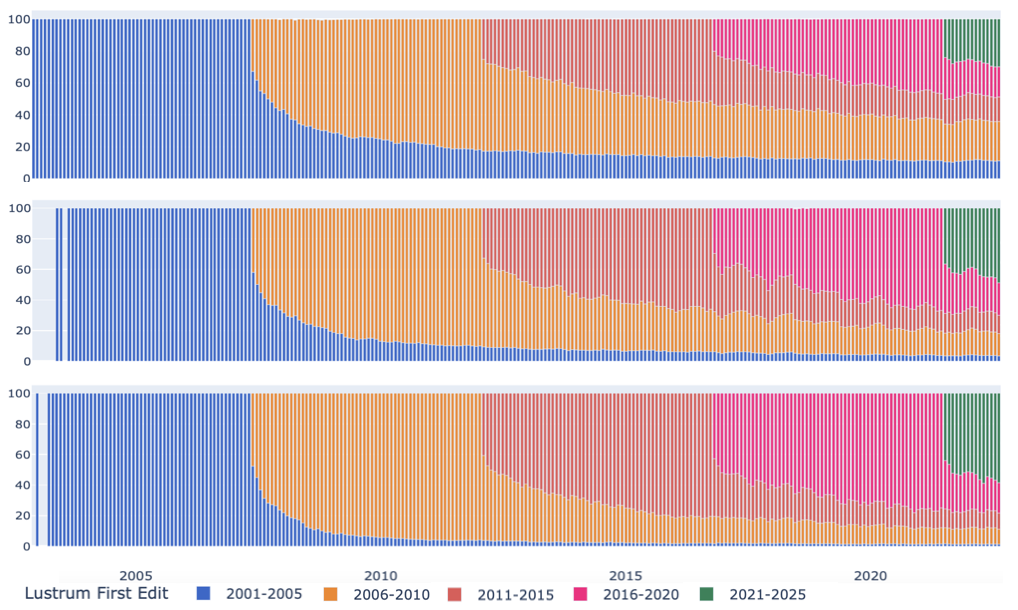
\includegraphics[width=470px]{img/balance_trend1.png}
    \setlocalecaption{english}{figure}{Figure}
    \caption{Trend of the major European languages' balance among active editors}
    \label{fig:balance_trend}
\end{figure}

In Figure \ref{fig:balance_trend} above we find, from top to bottom, Italian, German, French and Spanish.\\
There is a recurrent pattern: through the years, the new generations overtake the old ones, but not entirely. A generation is considered to be 5 years long.\\
The last generation (2021-2025) should occupy from 10 to 40\% depending on the years which have passed since its beginning, while the oldest generation (2001-2005) share should remain around 
5 to 15\%, not greater, to guarantee the generational change.

\section{Special functions}
\label{sec:special_conclusion}

Special functions are about editors which hold a certain role that allows them to perform special actions in Wikipedia. In particular, we have two distinct roles: Technical functions and Community coordination functions. We now analyze them both.

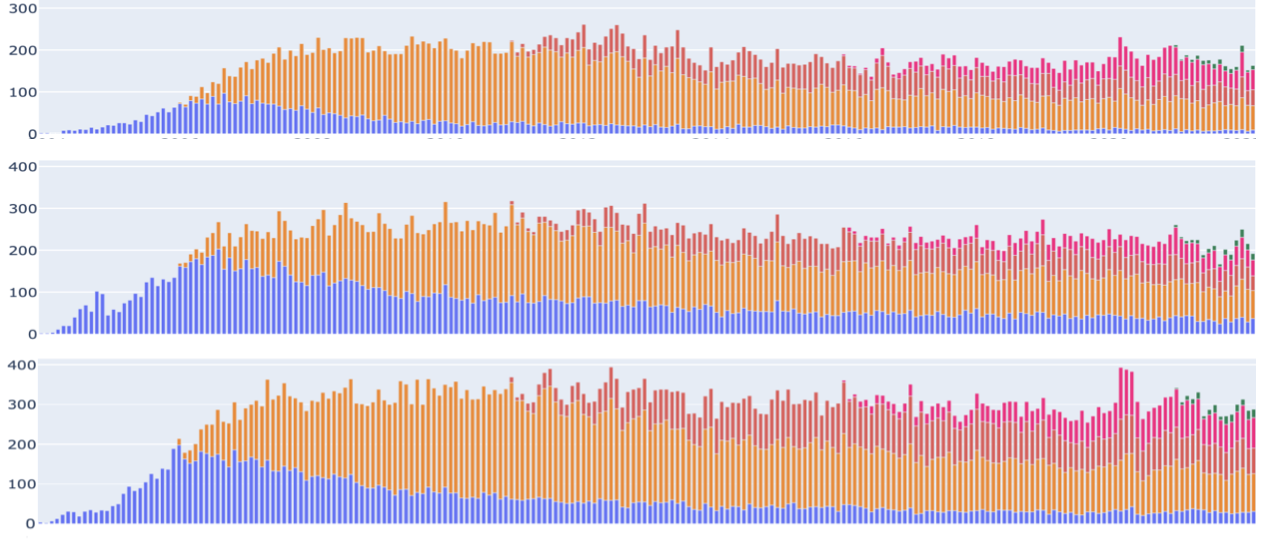
\includegraphics[width=470px]{img/tech_trend.png}
\begin{figure}[h]
    \centering
    
    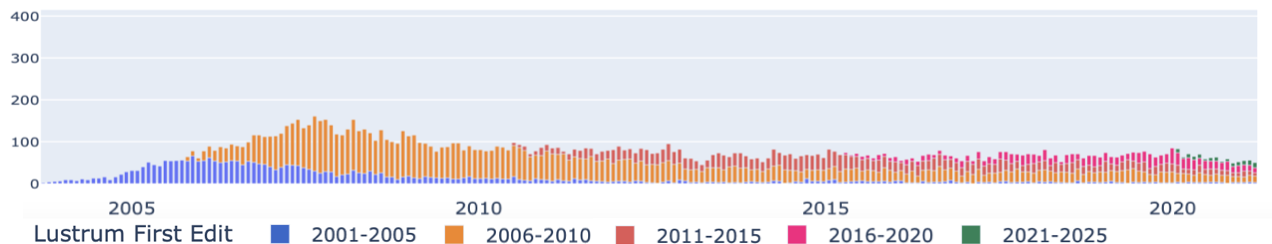
\includegraphics[width=470px]{img/tech_trend1.png}
    \setlocalecaption{english}{figure}{Figure}
    \caption{Trend of the major European languages' technical active editors}
    \label{fig:tech_trend}
\end{figure}
\pagebreak
\\
First we have technical editors. The majority of the them belongs to the 2006-2010 generation. The last generation 2021-2025 struggles at finding his space even if the older generation are now retreating.  From the Figure \ref{fig:tech_trend} we can clearly see that among active editors the color representing the second generation is significantly more present than the other generations. If we consult the online dashboards, we discover that, regardless of the editors being active or very active, this trend is consistent. Furthermore, it is a common pattern across different languages.

\begin{figure}[h]
    \centering
    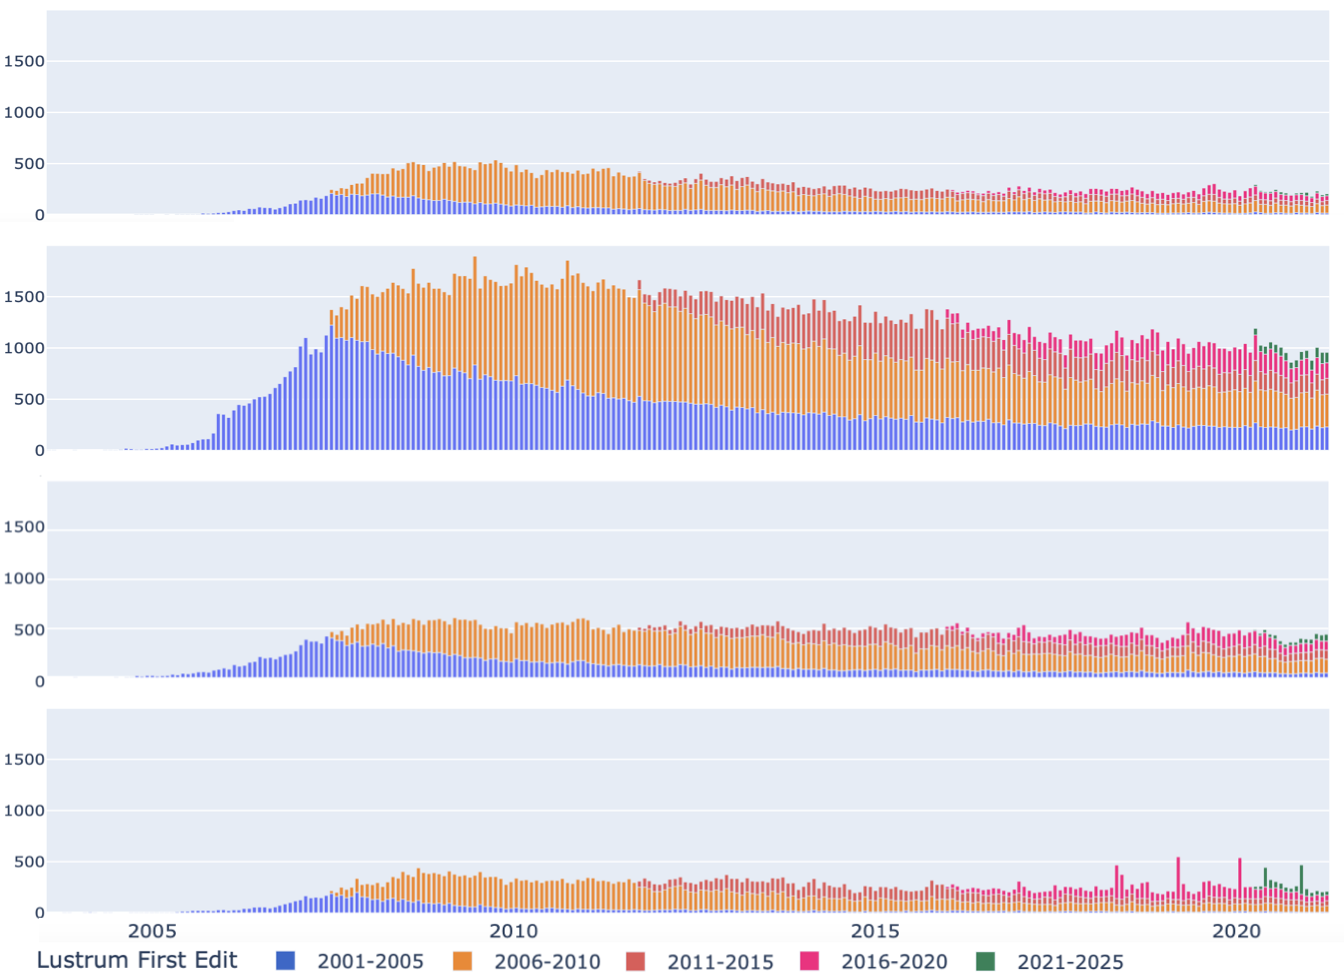
\includegraphics[width=470px]{img/coord_trend.png}
    \setlocalecaption{english}{figure}{Figure}
    \caption{Trend of the major European languages' coordinator active editors}
    \label{fig:coord_trend}
\end{figure}

Then we talk about coordinators. There are fewer and fewer new coordinators. As shown before when discussing technical editors, this trend is more evident among active editors visualizations, as we can see the color representing the second generation is more present than the other.\\
These trends could be the symptoms of a lesser interest in the specific functions of Wikipedia from the editors.\\
As before, we recommend to consult the online dashboard for a visualization taking in account both type of editors.

\section{Admin flags}
\label{sec:admin_conclusion}

We now observe the admin flags distribution among our language sample. This time the result is independent from the type of editors because it is function-specific. For this example, we only consider the ``sysop" flag since it is the most paradigmatic one among the admin flags.

\begin{figure}[h]
    \centering
    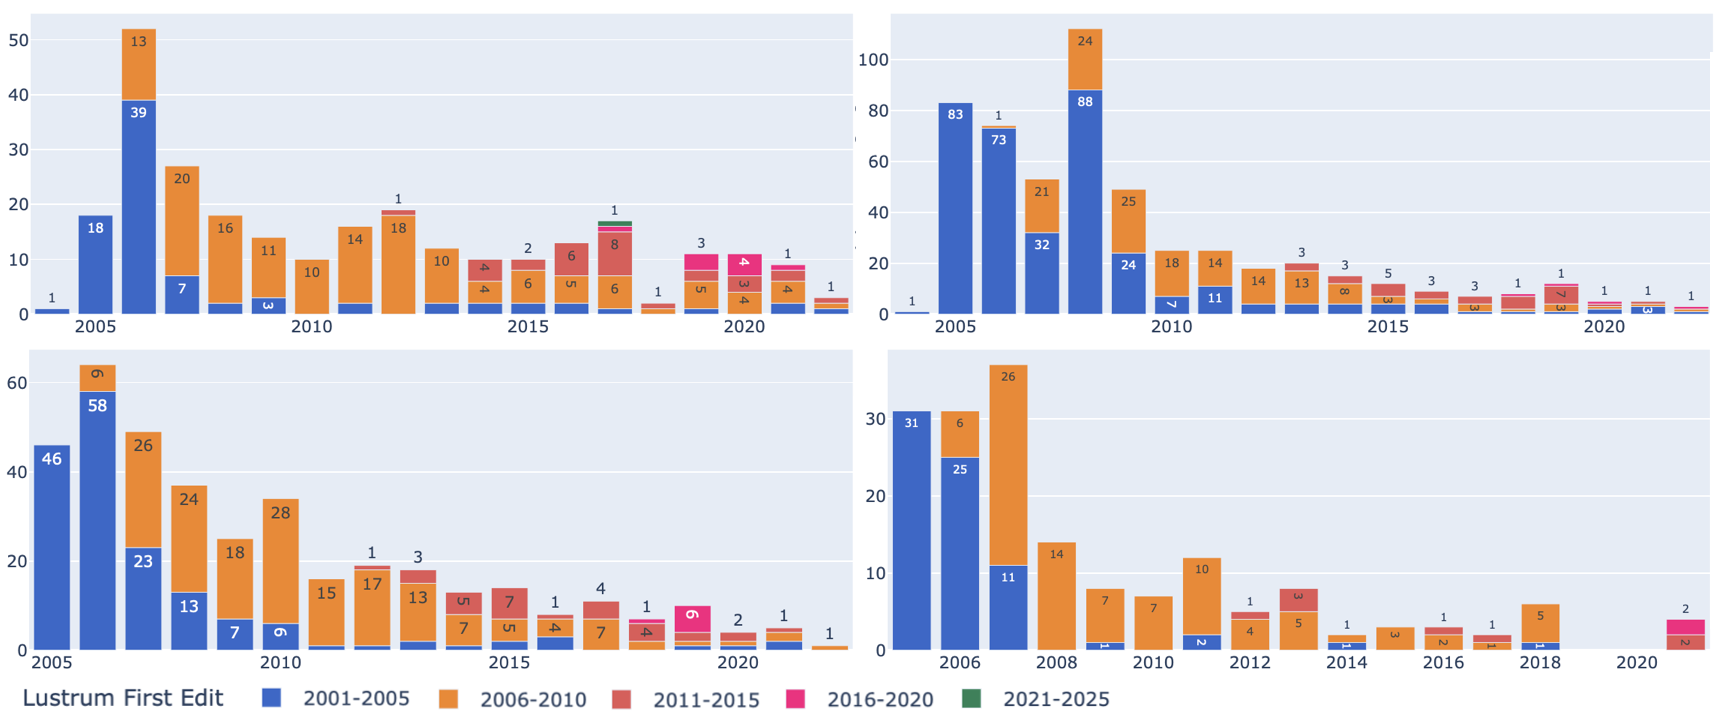
\includegraphics[width=470px]{img/admin_trend.png}
    \setlocalecaption{english}{figure}{Figure}
    \caption{Trend of the major European languages' admin distribution}
    \label{fig:admin_trend}
\end{figure}

In clockwise order we find Italian, German, Spanish and French.\\
Admin flags were given mainly in the past, especially to the first and second generation's editors.\\
In general, the percentage of a given admin flag, among active and very active editors, is borderline between being below and inline with the desired target of 1-5\%.

\section{Global community participation}
\label{sec:global_conclusion}

Finally we discuss the trend emerging from the global community. These trends are as important as the others since they move the focus on the bigger picture regarding the Wikipedia project as a whole. \\

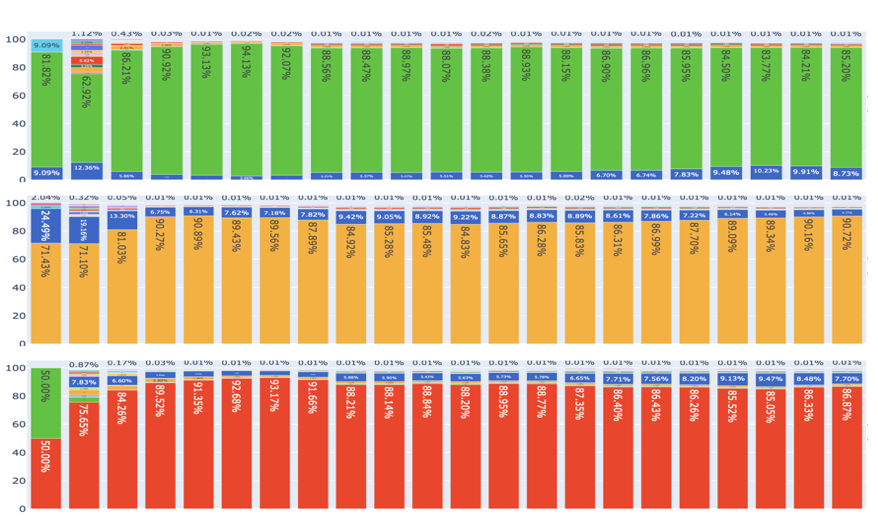
\includegraphics[width=470px]{img/global_trend.png}
\pagebreak
\begin{figure}[h]
    \centering
    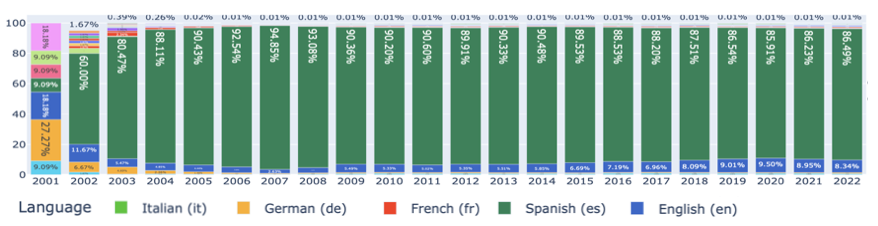
\includegraphics[width=470px]{img/global_trend1.png}
    \setlocalecaption{english}{figure}{Figure}
    \caption{Trend of the major European languages' global contribution}
    \label{fig:global_trend}
\end{figure}

From Figure \ref{fig:global_trend}, this time with a yearly time aggregation, we can see that the majority of the contributions for a given community come mainly from their primary language editors. In fact, the higher percentage has the same color of the analyzed language. However, the English community contributes consistently to every analyzed language. \\
We can observe a stabilizing trend: considering Italian and Spanish Wikipedia, in their early days they had different contributors that were, in percentage, much more active than today. Over the years, the minor communities percentage contribution decreased drastically, due to the affirmation of the big language community like German and English Wikipedia. Thus we can conclude that we lost diversity in the global contributions.This trend is inevitable, but the WikiCHM projects recommend the small community to keep editing in order to preserve their role in the global community.

\begin{figure}[h]
    \centering
    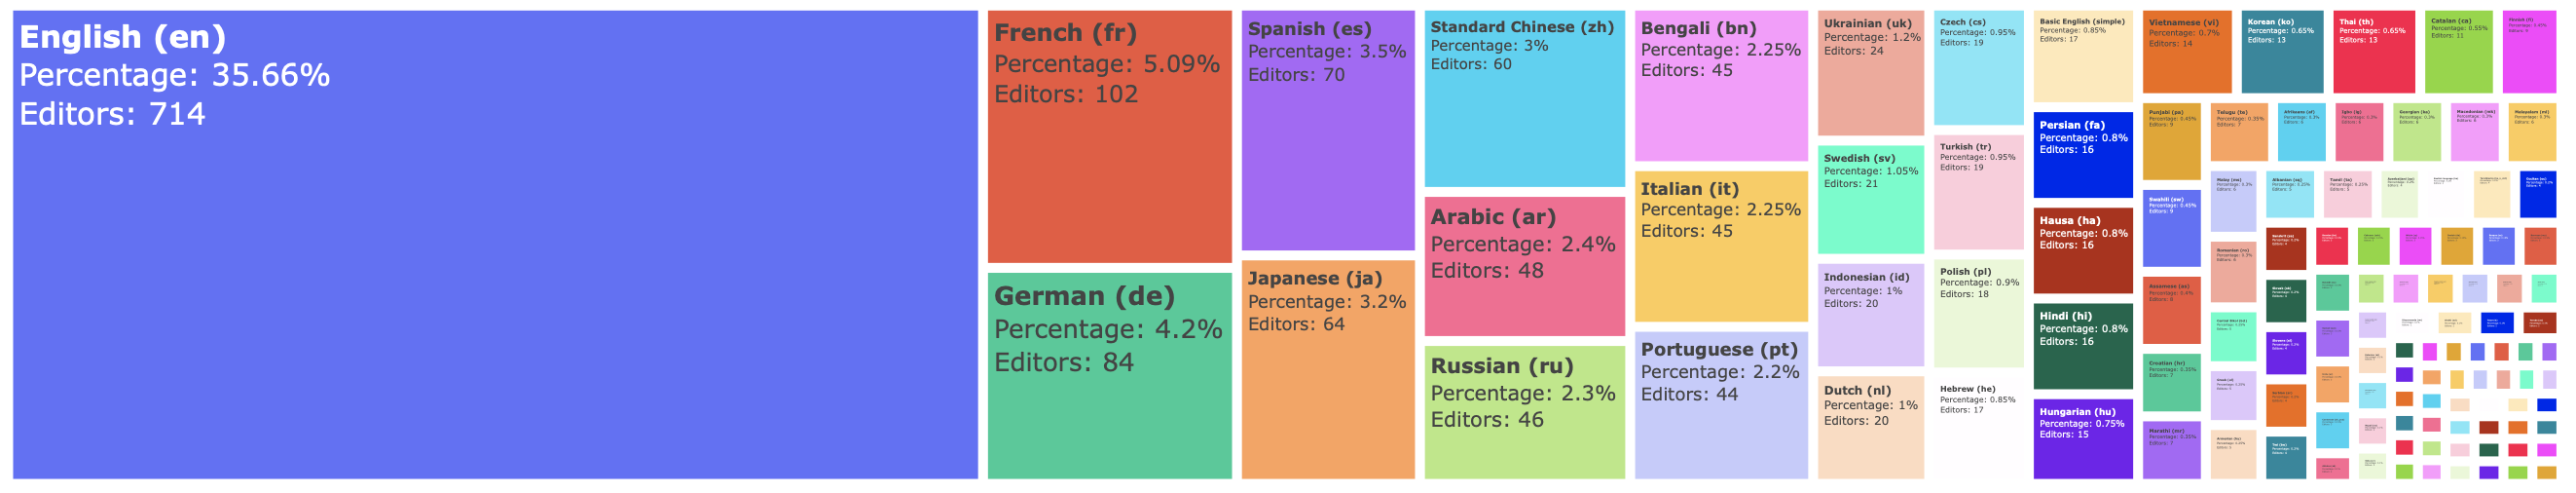
\includegraphics[width=470px]{img/meta_trend.png}
    \setlocalecaption{english}{figure}{Figure}
    \caption{Meta-wiki global participation }
    \label{fig:meta}
\end{figure}

Now we discuss the contribution of each language to the Meta-wiki. It is clear that the bigger language play a major role than the smaller ones. The English Wikipedia is the bigger contributor to the project, followed by other common languages like German, French but also Japanese and Chinese. \\
This result is extremely interesting since it shows that the European languages are not alone in the global Meta-wiki project, but there are the Asian giants too: the Japanese and Chinese community contributions reach, respectively, the 3.2\% and the 3\%; while the Arabic and Russian Wikipedia make their way among the big communities with, respectively, the 2.4\% and the 2.3\%.

